\documentclass[journal]{IEEEtran}
\usepackage{amsmath,amssymb}
\usepackage{booktabs,multirow,graphicx}
\usepackage{array,url}
\usepackage[hidelinks]{hyperref}
\hypersetup{pdftitle={Auditing Source-Label-Only Route Selection for Cross-Orbit Remaining-Useful-Life Prediction},pdfauthor={Author metadata pending confirmation}}
\emergencystretch=2em
\title{Auditing Source-Label-Only Route Selection for Cross-Orbit Remaining-Useful-Life Prediction}
\author{Author names, affiliations, and corresponding-author details pending confirmation}
\begin{document}
\maketitle

\begin{abstract}
Cross-orbit remaining-useful-life (RUL) studies can overstate transfer performance when repeated candidate revisions inspect the same outer outcomes. We specify and audit a source-label-only route-selection protocol for simulated battery (BAT) and reaction-wheel assembly (RWA) telemetry, while explicitly allowing target-orbit metadata and each target unit's earliest unlabeled window at inference. The audit found that the historical six-fold sequence informed successive revisions; those outcomes are therefore development diagnostics, not independent confirmation. A candidate and route were then frozen before one evaluation on a separately registered LEO600 partition. Against a same-partition frozen HGB/MLP reference, BAT's observed RMSE and MAE each decreased by about $9.53\times10^{-6}$ and $9.13\times10^{-6}$ cycles over five units and 125 windows. RWA tied on one usable unit and one window. These tiny, partition-specific differences pass a deterministic tolerance gate but do not establish statistical significance, practical relevance, or population generalization. We provide the data and split contract, executable method specification, hash-linked metrics, and production checks to make the evidence independently auditable.
\end{abstract}
\begin{IEEEkeywords}
remaining useful life, domain shift, prognostics, temporal convolutional network, evaluation protocol, reproducibility
\end{IEEEkeywords}

\section{Introduction}
RUL models are often evaluated as if training and test data shared one stable operating distribution. Changes in operating condition can instead alter the relationship between telemetry and residual lifetime. A route that improves an average source score can regress in one transfer direction, and repeated model revisions can silently turn an outer evaluation set into development data. Both problems are acute when the expected gains are close to floating-point or aggregation tolerances.

This study concerns two internally generated simulation streams, BAT and RWA, registered under the public BRPHM ModelScope dataset. It audits an existing source-label-only selection process and one frozen candidate on a separate LEO600 simulator partition. The final candidate uses a temporal convolutional network (TCN) blended with a frozen segmented histogram-gradient-boosting/multilayer-perceptron (HGB/MLP) control. It consumes the target unit's earliest unlabeled telemetry window and orbit identity. Accordingly, the evaluated information regime is label-free target-input/transductive; it is not pure inductive transfer.

The review identified a contradiction between the earlier claim of one-time outer evaluation and a sequence of six-fold failure counts that changed as candidates were revised. Chronology evidence now establishes that the historical outcomes belong to development. They are preserved for diagnosis and excluded from confirmatory claims. A new partition was frozen before its labels were accessed and evaluated once. This replacement evaluation is small and simulator-bounded; the paper does not present it as proof that the candidate is a generally successful domain-generalization method.

The contributions are:
\begin{itemize}
\item We provide an immutable chronology disposition for a reused outer-fold sequence and bind a separately frozen LEO600 evaluation to its manifest, event chain, candidate, and receipt hashes.
\item We formalize the model's actual information set, preprocessing, route equation, source gate, projection order, and deterministic implementation so that source-label use is distinguishable from unlabeled target-input use.
\item We release unit-level split membership, replayed tensor contracts, unrounded fold metrics, and source-gate diagnostics with explicit hashes and statistical limits.
\item We quantify what the replacement partition supports: a numerically tiny BAT gate gain and an RWA tie on one observation, with no inferential or population-wide claim.
\end{itemize}
No claim is made that the proposed candidate outperforms recent domain-adaptation methods. The available experiments do not provide a fair, same-data implementation comparison with those methods. Section~\ref{sec:related} distinguishes their information regimes and scope.

The remainder is organized as follows. Section~\ref{sec:related} reviews RUL transfer literature. Section~\ref{sec:data} specifies the dataset and split. Section~\ref{sec:method} defines the model and selection protocol. Sections~\ref{sec:results} and~\ref{sec:stats} report deterministic and statistical evidence. Sections~\ref{sec:audit}--\ref{sec:conclusion} cover reproducibility, limitations, and conclusions.

\section{Related Work}\label{sec:related}
RUL transfer methods address operating-condition changes through subdomain alignment, adversarial objectives, multisource adaptation, and online/self-supervised adaptation. Ding et al. study deep subdomain adaptation under multiple operating conditions in IEEE Transactions on Instrumentation and Measurement (TIM)~\cite{ding2021tim}. Li et al. use a transformer for domain-adaptive RUL prediction and report unlabeled-target alignment~\cite{li2022tim}. Wu et al. use weighted adversarial adaptation with target pseudo-labels~\cite{wu2022tim}. Ragab et al. study contrastive adversarial domain adaptation for machine RUL~\cite{ragab2021tii}; Ding et al. address multisource transfer across operating conditions~\cite{ding2022tmech}; and Mao et al. study self-supervised online adaptation under unknown bearing conditions~\cite{mao2023tii}.

These works establish direct prior art for RUL under condition shift. Their datasets, model objectives, and target information differ from the present registered simulation protocol. In particular, pseudo-label, unlabeled-target alignment, online-update, and multisource methods cannot be ranked fairly against this fixed candidate from the currently retained receipts. The comparison here is with one frozen segmented HGB/MLP control, not a state-of-the-art leaderboard. The present contribution is therefore an audit and reproducibility record for a specific evaluation contract, not a claim of algorithmic novelty or superiority over the cited methods.

\section{Data and Evaluation Contract}\label{sec:data}
\subsection{Dataset, version, and units}
The registered source dataset is \texttt{SIM\_bat} and \texttt{SIM\_rwa} in the public ModelScope repository \url{https://www.modelscope.cn/datasets/modelscope1553926531/BRPHM-datasets}. We pin commit \texttt{85ebba12\allowbreak f3ec132d\allowbreak c9e0ea8a\allowbreak e49012f5\allowbreak 7505ccf1}; the access date is 2026-10-02. The complete-tier tree and manifest match the observed current head, but the repository root manifests differ. The platform API declared CC-BY-4.0 on the access date; neither inspected commit contains a versioned license file, so applicability to the pinned historical commit is not commit-authenticated. No DOI was disclosed by the inspected API/README or found in the date-stamped exact-title searches. The analyzed SIM partitions are described as internally generated simulation; this paper does not assign the API license to unrelated collection partitions.

Raw main telemetry is sampled on a 10-s grid (0.1 Hz); available event details use 1-Hz windows around events. Registered units are split before windowing. Holdout assignment uses the configured 15\% fraction, nearest-integer rounding, seed 20260715, DOE-cell stratification, and a per-cell cap of one. Remaining units use a cell-tail split: sort by SHA-256 of \texttt{"0:<unit\_id>"}, assign the final $\mathrm{clamp}(\lfloor0.2n\rfloor,1,n-1)$ units to validation for $n>1$, and assign a singleton to training. Holdout membership takes precedence. No unit crosses splits.

\begin{table*}[t]
\centering
\caption{Registered source data and unit split counts. Window counts refer to processed train/validation tensors; registered holdout units are absent from these tensors.}
\label{tab:data}
\scriptsize
\resizebox{\textwidth}{!}{%
\begin{tabular}{llrrrrrr}
\toprule
Component & Orbit & Train units & Validation units & Holdout units & Train windows & Validation windows & Input contract \\
\midrule
BAT & LEO500 & 65 & 27 & 16 & 954 & 423 & 4 channels, $L=60$, stride 5 \\
BAT & LEO550 & 66 & 27 & 15 & 803 & 375 & 4 channels, $L=60$, stride 5 \\
BAT & LEO700 & 63 & 27 & 18 & 607 & 519 & 4 channels, $L=60$, stride 5 \\
RWA & LEO500 & 61 & 27 & 20 & 1610 & 742 & 13 channels, $L=30$, stride 1 \\
RWA & LEO550 & 63 & 27 & 18 & 1664 & 660 & 13 channels, $L=30$, stride 1 \\
RWA & LEO700 & 70 & 27 & 11 & 1610 & 765 & 13 channels, $L=30$, stride 1 \\
\bottomrule
\end{tabular}
}%
\end{table*}

BAT channels are capacity (Ah), internal-resistance proxy (ohm), mean temperature (C), and charge time (s). Its resistance proxy is explicitly absent-allowed and uses identity normalization, yielding zero when absent. RWA's 13 channels comprise mean, standard deviation, minimum, and maximum of three base telemetry channels, plus mean friction torque; the daily aggregation bin is 574 s. Both pipelines mean-impute missing values using training-split statistics; singleton-bin standard deviations are imputed with the training statistic. Negative RUL labels are dropped. Raw RUL is $T_f-t$; right-censored records have no failure time, a missing raw RUL, and a zero failure indicator. Normalization statistics are fitted on training units only and reused for validation. The hashed split membership file identifies all 648 registered units: 324 per component, 216 per orbit, 388 train, 162 validation, and 98 holdout. The processed payloads contain 3,681 BAT windows of shape $[3681,60,4]$ and 7,051 RWA windows of shape $[7051,30,13]$, with zero registered holdout units. Of train/validation units, 72 BAT and 35 RWA units have no valid windows and are not represented in those tensors.

\subsection{Separate final partition}
The replacement partition is a separately registered simulated LEO600 orbit, generated after the original outer-reuse issue was identified. Its manifest lists six raw units per component. One BAT unit is censored; under the frozen window/label contract, the final metric set contains five BAT units and 125 windows, and one RWA unit and one window. It is not part of the 648-unit source split. The partition manifest SHA-256 is \texttt{910c0582\allowbreak bc7e4513\allowbreak 85faccc4\allowbreak 8987f1cd\allowbreak b5b5684b\allowbreak a2b105ef\allowbreak a240a1e8\allowbreak f5ce3123}; the associated input tensor hashes and unit IDs are in the machine-readable F1 manifest. The simulated orbital period is approximately 5819 s, compared with the model tile period of 5740 s, a difference of about 79 s (approximately 608 km in the recorded audit). This mismatch limits physical interpretation.

The unit-membership CSV SHA-256 is \texttt{f07ac79a\allowbreak 69986b40\allowbreak 7b3af045\allowbreak 8201be99\allowbreak 3a2a0956\allowbreak d59ba7af\allowbreak 24abd028\allowbreak a14a24d}. The BAT and RWA processed tensor SHA-256 values are \texttt{9e2a7f3d\allowbreak bf22e99b\allowbreak 4685ff27\allowbreak 51c94e96\allowbreak 312d3800\allowbreak 32270771\allowbreak f7e29a51\allowbreak e30057ab} and \texttt{9dcbd45d\allowbreak 668cc030\allowbreak 89ef6280\allowbreak 68d1247e\allowbreak b2100f64\allowbreak b70c3d5b\allowbreak 4aba8ff2\allowbreak 62813595}, respectively. The train/validation replay was bitwise equal and traced zero holdout Parquet reads. The full manifest and split membership CSV are included in the reproduction bundle.

\subsection{Metrics}
For physical RUL $r_i$ and prediction $\hat r_i$, we compute window-weighted
\begin{equation}
 \begin{aligned}
 \mathrm{RMSE}&=\sqrt{n^{-1}\sum_i(\hat r_i-r_i)^2},\\[-1pt]
 \mathrm{MAE}&=n^{-1}\sum_i|\hat r_i-r_i|.
 \end{aligned}
\end{equation}
BAT is reported in cycles and RWA in days. Deltas are candidate minus reference, so a negative value is a lower error. All gate decisions use unrounded values; displayed values do not replace the hash-linked machine records.

\section{Method and Selection Protocol}\label{sec:method}
\subsection{Problem and information set}
For component $c$, each example is a window $X_i\in\mathbb{R}^{L_c\times C_c}$ with unit $u_i$, end time $t_i$, orbit $o_i$, and normalized label $y_i=r_i/r_{\max,c}\in[0,1]$. Here $(C_{\mathrm{BAT}},L_{\mathrm{BAT}},r_{\max,\mathrm{BAT}})=(4,60,150\ \mathrm{cycles})$ and $(C_{\mathrm{RWA}},L_{\mathrm{RWA}},r_{\max,\mathrm{RWA}})=(13,30,0.2\ \mathrm{days})$. The model representation has $2C_c$ channels: 8 for BAT and 26 for RWA.

Training and route selection use source labels. At inference, the implementation also reads the target orbit identity from unit metadata and the earliest unlabeled target window, selected by minimum window-end time, to construct unit-relative features. It does not read target RUL labels for fitting, route selection, residual correction, or thresholding. Thus the implemented setting is label-free target-input/transductive. Pure inductive transfer without target identity or target history is neither implemented nor evaluated.

\subsection{Representation and TCN}
For each source transfer, channel means and standard deviations are fitted over source windows only; a scale below $10^{-6}$ is floored at $10^{-6}$. After standardization, for each unit $u$ let $\tilde x_{u,0}$ be the first time point in the window with minimum end time. We concatenate
\begin{equation}
 z_{u,j,:}=\left[\tilde x_{u,j,:},\;\tilde x_{u,j,:}-\tilde x_{u,0,:}\right].
\end{equation}
This gives $z_u\in\mathbb{R}^{L_c\times 2C_c}$. A normalized age feature $a_i$ is formed from the unit's window-end time using the implementation's $10^{-9}$ denominator floor; the prediction head receives $a_i$, $a_i^2$, and $\sqrt{\max(a_i,0)}$.

The network transposes the input to channel-first order, applies a $1\times1$ convolution $2C_c\to16$, then three residual blocks with dilation $(1,2,4)$. Each block contains two width-16, kernel-3 convolutions with symmetric dilation padding; each convolution is followed by GroupNorm(1,16), SiLU, and dropout 0.05 before residual addition. The temporal last state and temporal mean are concatenated (32 features), then concatenated with the three age features. The head is $35\to16$ with SiLU, then $16\to1$ with sigmoid output. The age feature is $a_i=t_{i,\mathrm{end}}/\max(t_{\max,\mathrm{source}},10^{-9})$, where $t_{\max,\mathrm{source}}$ is the maximum source-window end time used when fitting that model. The nominal receptive field is 29 samples. Symmetric padding makes this network non-causal. Parameter count is $32C_c+5505$ (5,633 BAT; 5,921 RWA).

For each fixed seed in $(17,42,73)$, Python, NumPy, and PyTorch seeds are set; PyTorch default module initialization is used. We train exactly 90 epochs with AdamW (learning rate 0.002, weight decay $10^{-4}$), batch size $\min(256,n)$, a seeded shuffled data loader, SmoothL1 loss with $\beta=1$, and gradient norm clipping at 1.0. Each window has inverse-unit-window-count weight, rescaled so weights sum to $n$. There is no early stopping. Three prediction arrays are combined elementwise by their median.

\subsection{Residual correction, projection, and route}
The source-fit residual correction is $-0.25\,\mathrm{median}(\hat y_{\mathrm{src}}-y_{\mathrm{src}})$, computed on fitted source windows and frozen before transfer evaluation. Candidate predictions are corrected, then projected and clipped to $[0,1]$: BAT uses a non-increasing isotonic projection; RWA uses a causal running minimum. The frozen segmented HGB/MLP control uses the same component-specific final projection. For transfer direction $d=s\to t$ and target-orbit weight $\alpha_t$,
\begin{equation}
 q_d=\alpha_t p_{\mathrm{candidate},d}+(1-\alpha_t)p_{\mathrm{control},d}.
\end{equation}
Here $\alpha=0$ is control-only and $\alpha=1$ is candidate-only. The formal path blends the already projected candidate and control, then reapplies the component projection and clipping before metrics.

The registered route catalog is the five-family/64-mask contract
\begin{equation*}
\begin{aligned}
 \mathcal A={}&\{(0,0.5),(0.1,0.5),(0.25,0.5),\\[-1pt]
 &\quad(0.1,0.25),(0.25,0.75)\}.
\end{aligned}
\end{equation*}
where each family assigns its low or high value to each of the six directed source transfers. It therefore contains $5\times2^6=320$ routes with IDs `family\textit{i}\_mask\textit{m}`. The source gate requires complete RMSE/MAE records for six directed transfers and residual-KS records for three orbit pairs. A route is rejected if any source RMSE, MAE, or KS statistic regresses by more than $10^{-12}$ relative to control; it must also have at least one strict RMSE/MAE gain below $-10^{-12}$. Among eligible routes, the registered conservative selector and the uniform-floor rule are frozen from the source receipt; every promoted target alpha is at least $10^{-5}$. Among eligible routes, the lexicographic key is ordered as
\begin{equation*}
\begin{aligned}
K(r)&=\bigl(\textstyle\sum_o\alpha_o,\ \max_o\alpha_o,\ \mathrm{worstKS}(r),\\[-1pt]
&\quad \mathrm{meanRMSE}(r),\ \mathrm{meanMAE}(r),\ r_{\mathrm{id}}\bigr).
\end{aligned}
\end{equation*}
For the unseen LEO600 target, the frozen rule assigns $\alpha=10^{-5}$ for both components. The historical 17-point/4913-route catalog is retained only as development/diagnostic evidence and is not the final selection contract.

\subsection{Executable procedure and cost}
\noindent\textbf{Procedure.} (1) Verify unit-disjoint source/validation membership and tensor hashes. (2) Fit the source-only scaler. (3) Append per-unit earliest-window relative channels. (4) Fit the three fixed-seed TCNs; take the median and apply the frozen source-residual correction. (5) Project candidate and control predictions. (6) Enumerate the 320 registered family/mask routes, apply the source gate and conservative selector, and freeze the selected route. (7) Freeze the candidate, source artifacts, and final partition manifest before final-label access. (8) Evaluate once, blend projected predictions with the preassigned unseen-orbit alpha, reproject, compute metrics, and write a hash-bound receipt.

For $N$ windows, sequence length $L$, raw channels $C$, width $W=16$, three blocks, and kernel $k=3$, the dominant per-epoch cost is $O(NL(2CW+2\cdot3W^2k))$. The three-seed 90-epoch fit multiplies this term by 270; activation memory is $O(\min(256,N)L(2C+W))$ plus model parameters. The implementation rejects empty source sets, nonfinite arrays, rank/channel mismatches, incomplete transfer grids, and source/validation unit overlap. Constant source channels use the scale floor; one-window units are valid, and their adjacent-step monotonicity fraction is undefined.

\section{Chronology and Development Diagnostics}
\subsection{F1 disposition}
The immutable record does not support the original claim that outer outcomes were never visible during candidate development. The historical successive-candidate fold-failure counts $5,4,3,1,3,0$ are all classified as development/diagnostic because later revisions followed those outcomes and a complete contemporaneous outer-read/selection log is unavailable. The uniform floor is therefore not presented as an untouched six-fold confirmation. A new LEO600 candidate snapshot and route were frozen before the final label-access event; the separate partition was then evaluated once. The receipt hash is \texttt{3eff57fe\allowbreak 0703fc85\allowbreak 1e8a96c0\allowbreak 01666003\allowbreak 4fc72c30\allowbreak d2e20b3c\allowbreak 3de220c6\allowbreak 893ce459}. Event hashes, timestamps, selection decision, and remaining historical-log gaps are listed in the F1 evidence ledger.

\subsection{Historical candidate matrix}
Table~\ref{tab:progression} preserves the complete reported denominator. It is diagnostic only; GRU's dash means not eligible and is never interpreted as zero.
\begin{table}[t]
\centering
\caption{Historical sequence; all outer-fold counts are development/diagnostic after F1.}
\label{tab:progression}
\scriptsize
\resizebox{\columnwidth}{!}{%
\begin{tabular}{lccc}
\toprule
Candidate & BAT source gate & RWA source gate & Outer folds regressed / 6 \\
\midrule
Unit-first TCN & pass & pass & 5/6 \\
Residual-centered & pass & pass & 4/6 \\
Residual-centered L1 & pass & pass & 3/6 \\
L1 worst-direction & pass & pass & 1/6 \\
RWA LEO550 floor & pass & pass & 3/6 \\
Uniform alpha floor & pass & pass & 0/6 \\
GRU & fail & fail & N/A (ineligible) \\
\bottomrule
\end{tabular}%
}
\end{table}
Adjacent source-gate variants changed one declared factor at a time, but the historical sequence was informed by reused outer results. It is not an independent controlled confirmation. Full candidate-by-fold and source-gate matrices, including the six directed transfers, three KS pairs, sample counts, statistics, and p-values, are supplied as CSV. The GRU failed its source gate and did not enter formal evaluation.

\begin{figure}[t]
\centering
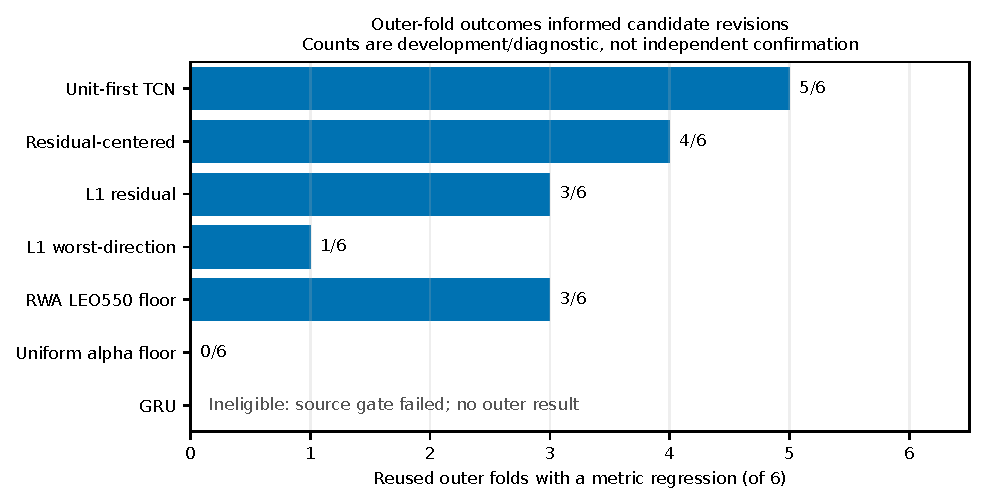
\includegraphics[width=\columnwidth]{../figures/method_progression.pdf}
\caption{Historical candidate progression shown only as development evidence. The plot reports counts out of six and labels the GRU ineligible rather than assigning it a numeric zero.}
\label{fig:progression}
\end{figure}

\section{Results}\label{sec:results}
\subsection{Historical six-fold metrics}
The six-fold values remain useful for debugging the source route but not as untouched confirmation. Table~\ref{tab:oldfold} reports exact window counts and high-precision deltas from the frozen reference. The complete reference and candidate RMSE/MAE values, per-unit CSV, and gate calculations are hash-linked in the F5 machine record. Reference hash: \texttt{b708df9c\allowbreak 448a051b\allowbreak 8669c297\allowbreak 89f00d28\allowbreak 2aa79077\allowbreak 84e6f99d\allowbreak 7e20ef1f\allowbreak b96b6733}. Candidate source receipt hash: \texttt{b99ed8a3\allowbreak d2f16848\allowbreak 3f1072e7\allowbreak 363fe179\allowbreak 3a08708c\allowbreak 16693ea6\allowbreak ba59e29b\allowbreak f03631f1}.
\begin{table*}[t]
\centering
\caption{Historical metrics retained as development/diagnostic evidence. Delta equals candidate minus reference; all calculations use unrounded values.}
\label{tab:oldfold}
\scriptsize
\resizebox{\textwidth}{!}{%
\begin{tabular}{llrrr}
\toprule
Component & Test orbit & Units / windows & $\Delta$RMSE (physical units) & $\Delta$MAE (physical units) \\
\midrule
BAT & LEO500 & 70 / 1377 & $-3.6567708308066216\times10^{-6}$ cycles & $-1.3458916285902234\times10^{-6}$ cycles \\
BAT & LEO550 & 68 / 1178 & $-9.5934971171551800\times10^{-6}$ cycles & $-3.9320056219871450\times10^{-6}$ cycles \\
BAT & LEO700 & 65 / 1126 & $-3.0063242983491280\times10^{-5}$ cycles & $-1.8591568749837250\times10^{-5}$ cycles \\
RWA & LEO500 & 78 / 2352 & $-2.5164912758831454\times10^{-5}$ days & $-5.2089244800476720\times10^{-7}$ days \\
RWA & LEO550 & 79 / 2324 & $-1.3337010568853502\times10^{-8}$ days & $-1.4887936734125917\times10^{-9}$ days \\
RWA & LEO700 & 83 / 2375 & $-2.9375295713257588\times10^{-8}$ days & $-2.1671621424496080\times10^{-8}$ days \\
\bottomrule
\end{tabular}%
}
\end{table*}

\subsection{One-time LEO600 evaluation}
The frozen final receipt contains five usable BAT units (125 windows) and one usable RWA unit (one window). The table reports receipt values directly; RWA's equal candidate/reference values are a tie on that one observation.
\begin{table}[t]
\centering
\caption{One-time LEO600 comparison after candidate freeze. These values are partition-specific and are not significance estimates.}
\label{tab:leo600}
\scriptsize
\resizebox{\columnwidth}{!}{%
\begin{tabular}{lrrr}
\toprule
Measure & Reference & Candidate & Delta \\
\midrule
BAT RMSE (cycles), 5 units / 125 windows & 1.1142966431138528 & 1.1142871129918521 & $-9.5301220006672\times10^{-6}$ \\
BAT MAE (cycles), 5 units / 125 windows & 0.6738513384014369 & 0.6738422054797410 & $-9.1329216958\times10^{-6}$ \\
RWA RMSE (days), 1 unit / 1 window & 0.005497685074806214 & 0.005497685074806214 & 0 \\
RWA MAE (days), 1 unit / 1 window & 0.005497685074806214 & 0.005497685074806214 & 0 \\
\bottomrule
\end{tabular}%
}
\end{table}

For this partition the deterministic gate required non-inferiority within $10^{-12}$ for both metrics on both components and at least one strict gain below $-10^{-12}$. The stored receipt records the gate as passed: BAT supplies the strict gain and RWA is tied. The BAT deltas are approximately $-0.000855\%$ RMSE and $-0.001355\%$ MAE relative to the same-partition control. These values are numerically small and do not by themselves show engineering relevance. No candidate, threshold, or route was selected from this final result.

\begin{figure}[t]
\centering
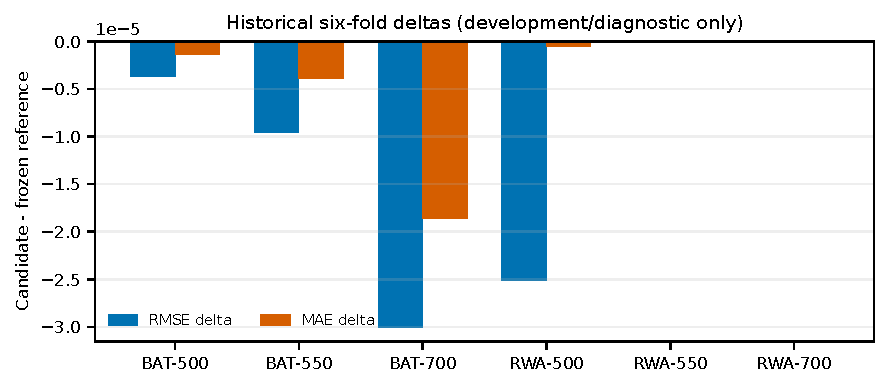
\includegraphics[width=\columnwidth]{../figures/formal_deltas.pdf}
\caption{Historical six-fold metric deltas retained for diagnosis only. All displayed observations belong to reused development folds.}
\label{fig:deltas}
\end{figure}

\section{Statistical Evidence}\label{sec:stats}
The six component-by-orbit folds are not six independent replications, and the three training seeds form a prediction ensemble rather than independent experimental repetitions. The F6 analysis therefore reports fold-specific descriptive results, seed sensitivity, and unit-cluster resampling; it does not treat folds or seeds as independent study replications.

For each historical fold, the candidate's complete unit clusters were resampled with replacement 20,000 times (seed 20261002), preserving all windows within each sampled unit. The frozen reference fold aggregate was held fixed because reference per-unit predictions were not retained. The analysis used one-sided 99.5833\% upper bounds with Bonferroni correction across 12 fold-by-metric comparisons (six folds times RMSE/MAE). The resulting bounds do not support familywise non-regression or strict gain; confidence intervals for candidate-minus-fixed-reference differences include zero. The fixed-reference bootstrap omits reference sampling variance and paired covariance, so it is not a paired treatment-effect analysis. A valid frozen-reference paired bootstrap/Wilcoxon test and practical-significance threshold are unavailable. The three-seed summaries and all fold/unit distributions are machine-readable and should be read as sensitivity diagnostics.

For the source gate, all six directed transfers and three residual-KS pairs are retained in \texttt{source\_gate\_matrix.csv}. It includes per-direction unit/window counts, RMSE/MAE and deltas, KS statistics, nominal window-IID p-values, the $10^{-12}$ gate threshold, and pass fields. Windows overlap within units; the nominal IID KS p-values are descriptive only. The unit-cluster permutation/bootstrap comparison in the F8 record is exploratory because route selection used the same source-validation directions. Its six corrected intervals include zero and its Holm-adjusted one-sided p-values equal 1. Thus those source diagnostics do not provide inferential evidence of improvement.

\section{Audit and Reproducibility}\label{sec:audit}
The F1 event chain records preflight, candidate freeze, final-label access, evaluation, and same-partition gate. The final receipt binds the candidate freeze manifest (SHA-256 \texttt{0e13d131\allowbreak ecf28d9f\allowbreak 867e823a\allowbreak 9387fd3e\allowbreak d3af3981\allowbreak 44d90c6a\allowbreak faf5cda2\allowbreak d1f04e69}), separate LEO600 manifest, selected route, per-component input/output payloads, and result. The receipt SHA-256 is \texttt{3eff57fe\allowbreak 0703fc85\allowbreak 1e8a96c0\allowbreak 01666003\allowbreak 4fc72c30\allowbreak d2e20b3c\allowbreak 3de220c6\allowbreak 893ce459}. The event chain and decision files are included under \nolinkurl{review/f1_leo600_final_retry1_20261002/}. Historical outer-read logs and exact old shell arguments were not preserved; this is why the old folds remain diagnostic.

The final receipt records Rack Linux x86\_64, kernel 6.8.0-110-generic, Python 3.10.20, NumPy 1.26.4, pandas 2.3.3, SciPy 1.15.3, scikit-learn 1.7.2, PyArrow 24.0.0, PyTorch 2.3.1, and execution device CPU. The host was an Intel Xeon Platinum 8473C with 208 logical CPUs and 251 GiB memory; these are host capacity figures, not a claim that the run consumed all resources. A separately queried preprocessing environment had a CUDA-enabled PyTorch build, but it was not the final evaluation device. The local PDF was built on Windows 11 with MiKTeX/Poppler; those are production-check tools, not model-training runtime.

Reproduction materials include the split manifest and unit-membership CSV; tensor replay addendum; F1 chronology and final receipt; F3 method, F4 route, F5 unrounded metrics, F6 statistics, and F8 source-gate records; source scripts; figure source; and this manuscript. The registered ModelScope data are not duplicated in the bundle. Exact data access and license boundaries are stated in Section~\ref{sec:data}. The current evidence package has local hashes; a permanent public artifact DOI and immutable release URL are not yet assigned.

\section{Limitations and Publication Declarations}
The one-time partition is narrow: five BAT units/125 windows and one RWA unit/one window on one simulated orbit. The BAT gain is tiny, the RWA comparison is only a one-window tie, and the simulator period differs from the model tile. Historical folds reused during candidate development cannot be used as confirmation. No fair implementation-level comparison with recent domain-adaptation methods is retained, and no pure-inductive result is available. These facts prevent a broad generalization or superiority claim.

\noindent\textbf{Funding:} author confirmation required.\\
\textbf{Conflict of interest:} author confirmation required.\\
\textbf{Author metadata:} names, affiliations, ORCIDs, and corresponding author require confirmation.\\
\textbf{Data availability:} the registered source dataset is at the ModelScope URL and pinned commit listed above; DOI not found in the audited metadata. The platform API declared CC-BY-4.0 on 2026-10-02, but commit-specific license applicability requires confirmation. The LEO600 simulator inputs and audit bundle are local research artifacts; a public immutable release remains to be prepared.\\
\textbf{Code availability:} the project repository is \url{https://github.com/1553926531-sudo/BRPHM}; the exact paper artifact release and commit are pending upload and hash verification.\\
\textbf{Privacy and ethics:} the analyzed streams are documented as generated simulations, not human or animal observations. Human/animal ethics review is therefore not applicable on the inspected data description. Authors must confirm data distribution permissions and that no personal or third-party telemetry is included.\\
\textbf{Venue and production:} IEEE TIM is the leading conditional venue candidate; no journal, article type, track, or official submission rule has been selected. Venue-specific template, length, blind-review, PDF eXpress, accessibility, and metadata requirements remain pending.

\section{Conclusion}\label{sec:conclusion}
This paper replaces an invalid one-time-evaluation narrative with an auditable chronology: the old six-fold sequence is development evidence, and the separately frozen LEO600 partition was evaluated once. We formalized the source-label route and its target-input information set, data contract, model, and machine-readable gates. The new partition yields a deterministic, very small BAT error reduction and an RWA tie on one observation; the cluster and fold analyses do not establish statistical improvement. The evidence supports a narrowly scoped reproducibility and evaluation report. Any stronger reliability, measurement, algorithmic-novelty, or population-generalization claim requires additional data and author-verified publication artifacts.

\begin{thebibliography}{00}
\bibitem{bai2018tcn} S. Bai, J. Z. Kolter, and V. Koltun, ``An empirical evaluation of generic convolutional and recurrent networks for sequence modeling,'' arXiv:1803.01271, 2018.
\bibitem{huber1964} P. J. Huber, ``Robust estimation of a location parameter,'' \emph{The Annals of Mathematical Statistics}, vol. 35, no. 1, pp. 73--101, 1964, doi: 10.1214/aoms/1177703732.
\bibitem{ben2010domain} S. Ben-David, J. Blitzer, K. Crammer, A. Kulesza, F. Pereira, and J. W. Vaughan, ``A theory of learning from different domains,'' \emph{Machine Learning}, vol. 79, pp. 151--175, 2010, doi: 10.1007/s10994-009-5152-4.
\bibitem{ding2021tim} Y. Ding, M. Jia, and Y. Cao, ``Remaining useful life estimation under multiple operating conditions via deep subdomain adaptation,'' \emph{IEEE Transactions on Instrumentation and Measurement}, vol. 70, pp. 1--11, 2021, doi: 10.1109/TIM.2021.3076567.
\bibitem{li2022tim} X. Li, J. Li, L. Zuo, L. Zhu, and H. T. Shen, ``Domain adaptive remaining useful life prediction with transformer,'' \emph{IEEE Transactions on Instrumentation and Measurement}, vol. 71, pp. 1--13, 2022, doi: 10.1109/TIM.2022.3200667.
\bibitem{wu2022tim} K. Wu, J. Li, L. Zuo, K. Lu, and H. T. Shen, ``Weighted adversarial domain adaptation for machine remaining useful life prediction,'' \emph{IEEE Transactions on Instrumentation and Measurement}, vol. 71, pp. 1--11, 2022, doi: 10.1109/TIM.2022.3212525.
\bibitem{ragab2021tii} M. Ragab, Z. Chen, M. Wu, C.-S. Foo, C. K. Kwoh, R. Yan, and X. Li, ``Contrastive adversarial domain adaptation for machine remaining useful life prediction,'' \emph{IEEE Transactions on Industrial Informatics}, vol. 17, no. 8, pp. 5239--5249, 2021, doi: 10.1109/TII.2020.3032690.
\bibitem{ding2022tmech} Y. Ding, P. Ding, X. Zhao, Y. Cao, and M. Jia, ``Transfer learning for remaining useful life prediction across operating conditions based on multisource domain adaptation,'' \emph{IEEE/ASME Transactions on Mechatronics}, vol. 27, no. 5, pp. 4143--4152, 2022, doi: 10.1109/TMECH.2022.3147534.
\bibitem{mao2023tii} W. Mao, J. Chen, J. Liu, and X. Liang, ``Self-supervised deep domain-adversarial regression adaptation for online remaining useful life prediction of rolling bearing under unknown working condition,'' \emph{IEEE Transactions on Industrial Informatics}, vol. 19, no. 2, pp. 1227--1237, 2023, doi: 10.1109/TII.2022.3172704.
\end{thebibliography}
\end{document}

